\section{Minimum violation planning}

\subsection{Problem significance}
Recent years have seen increased urbanization, economic expansion, underinvestment in infrastructure, and the rise of ride hailing services and e-commerce.  These changes have led to an increase in transportation delays, vehicle congestion during peak times, and environmental impacts resulting in escalating mobility challenges in urban areas. The emerging Urban Air Mobility (UAM) aviation market is being catalyzed by advances in increasingly autonomous systems, electric propulsion, and novel business models such as on-demand, aerial ride sharing, thereby helping to address congestion issues in urban areas~\cite{flightplan2030}.  

UAM has the potential to be a safe, functional solution to the air transportation problem for passengers and cargo in and around a densely populated urban area.  An air traffic management system that governs a large number of these novel UAM operations over a small geographical area in a safe and efficient fashion is key to the realization and deployment of the UAM vision.  The notion of on-demand, (near) point-to-point mobility that transits people or goods over congested urban areas offers the potential for reduced transit times, as well as decreased environmental impact, for low-noise, electrified UAM vehicles.  Note that due to the near point-to-point nature of the solution, UAM operations must be tightly integrated with local communities and existing modes of transportation. 


\subsection{Scalable and Verifiable Safety for UAM}
The scale and density of projected UAM operations will far exceed the safe workload capacity of human controllers, necessitating the deployment of increasingly autonomous solutions for functions like aircraft management (e.g., managing flightpath and altitude requests, managing airborne and ground based holding times, etc.) and aircraft separation.

Currently, there is no established infrastructure for air traffic management of a scalable UAM concept of operations. Under current aviation paradigms, air traffic management is carried out in a centralized fashion by air traffic controllers.  The U.S. National Airspace System (NAS) is comprised of 5.3 million square miles of domestic airspace and 24 million square miles of oceanic airspace.  There are approximately 5,000 flights airborne at any given moment.  Over 14,000 air traffic controllers manage these aircraft and perform multiple safety-critical functions, such as air traffic separation which guarantees that a minimum spacing between aircraft is maintained \cite{FAAData}.  In contrast, for UAM operations to deploy at scale for profit, it will be necessary to have hundreds (or even thousands) of UAM aircraft aloft over an urban airspace under 500 square miles~\cite{goyal2018urban}.  The sheer number of vehicles, along with the necessary reduced separation criteria between them in order to achieve the required densities, will require the development of increasingly autonomous capabilities for aircraft clearance, separation, and flow management in the UAM ecosystem.  

Deploying increasingly autonomous systems in the US airspace is a challenge. Commercial aviation is among one of the most safety-critical systems in the world and has stringent standards for the design, deployment, and operation of aircraft and air traffic control systems. These regulations are detailed in chapter 14 of the Code of Federal Regulations (14 CFR). The ability to assure increasingly autonomous systems to aviation grade standards is thus crucial for their acceptance.  Safety-critical functions such as aircraft separation must provide strict guarantees on their behavior and the correctness of their outcomes.  Thus, increasingly autonomous air traffic management systems will have to tackle the dual issues of scalability and verifiable safety in order to be deployed in the NAS.


\subsection{Setting}
 In this paper, we employ a hierarchical decomposition of the UAM operations space motivated by the physical and geographical infrastructure required to field the system. Such an architecture has been studied in~\cite{bhnfm,bhTCNS} and allows for scalable air traffic management.  UAM vehicles take off and land from a landing pad, called a vertipad, which includes the final approach and takeoff (FATO) area.  A vertiport is comprised of several vertipads, the respective vertipad FATOs, and charging and maintenance facilities.  A vertihub is comprised of several vertiports.  Vertihubs provide air traffic control services (i.e., real time control of aircraft movement) between vertiports under their control and air traffic management services (i.e., strategic and long term planning of aircraft movement and flows) for vehicles transiting between adjacent vertihubs.  Figure~\ref{fig:uam_architecture} provides a visual representation of vertiports and vertihubs.  We focus on a synthesis strategy for vertihubs, each of which is responsible for assuring the safety of all vehicles in its airspace.  


\begin{figure}
    \centering
    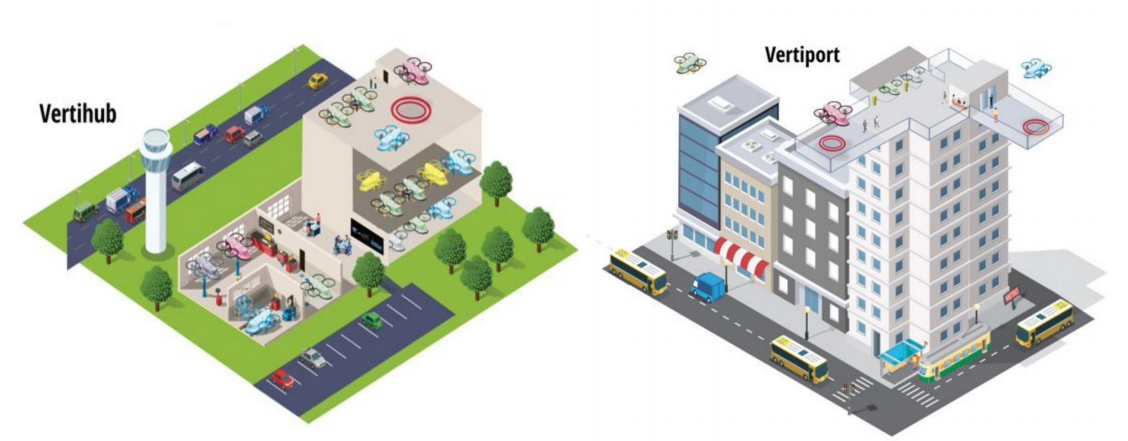
\includegraphics[width=0.98\columnwidth]{UAM-NFM/Figures/vert.PNG}
    \caption{Vertihub and vertiport depiction}
     \label{fig:uam_architecture}
\end{figure}

In general, it is not always feasible to guarantee the satisfaction of all safety constraints under all conditions. Such scenarios are explicitly accounted for in 14 CFR \S 107.21, which allows for emergency deviation from regulations if required as long as the deviation is reported. For example, a vehicle may have to make an emergency landing if it is about to run out of fuel, even if violates separation requirements. Thus, there is a need for an air traffic management approach that allows for \emph{formally justifiable} violation of safety constraints if necessary. In this paper, we study the synthesis of control strategies for automated air traffic management for UAM while obeying safety regulations. In particular, we focus on the case where all safety regulations cannot be feasibly satisfied, as is allowed for small, cargo-carrying UAS under emergency operation. We present a decentralized, scalable synthesis approach that provably \emph{minimally violates} the given safety requirements.  Note that if it is possible to satisfy all safety properties for the duration of the flight, the approach yields a solution with zero violations (i.e., all safety requirements are guaranteed for the duration of the flight). %\nok{I'm not sure where this would be an appropriate place to add but we should explicitly mention that in the case where all the requirements can be satisfied, our solution will indeed result in 0 violation. (There was the time when I gave a talk about minimum violation planning and a question like this came up, so it might not be obvious to everyone that by minimizing violation, we'll have 0 violation if all requirements can be satisfied.)}

\subsection{Contribution and Innovation}

We present the first decentralized approach to minimum violation planning. We use temporal logic for a formal representation of safety regulations and guarantee that these regulations are minimally violated across the global system. Furthermore, we establish a \emph{framework} in this paper for minimum-violation for the small UAS cargo-carrying application over urban areas. Our framework has the following properties:

\begin{itemize}
    \item \emph{Scalability} - UAM operations are envisioned to occur at a scale well beyond the capabilities of current air traffic management approaches, as current day approaches are typically labor-intensive. It is crucial to safely guarantee operations of increasingly autonomous vehicles at scale in order for UAM to be commercially viable. 
    
    \item \emph{Decentralization} - The environment is likely to encompass multiple service providers and stakeholders. Each stakeholder will have potentially competing priorities and requirements. Consequently, the full state of the entire system is unlikely to be controlled or even observed by a single entity.
    
    \item \emph{Transparency} - With companies ranging from startups to corporations developing UAM vehicles, services, and capabilities, there is a disconnect between regulation and the pace of technological development. Bridging the gap between regulation and real-world implementation practices is necessary for a viable path to deployment. 
    
    \item \emph{Flexibility} - The technological and regulatory landscape of UAM is rapidly changing. Any proposed framework that cannot efficiently incorporate a change in regulation or emerging capabilities is not a viable solution. 
    
    \item \emph{Auditability} - All violations of regulations must be formally accounted for and reported. Our proposed method implicitly allows for such an analysis, as it not only synthesizes a control strategy for air traffic management but also the associated violation. 
    
    % allows for \textit{a posteriori} analysis on runs of the system \nok{I'm not sure how to put this more accurately but we should mention that the framework implicitly incorporates analysis in that it does not only generate a plan but also the violation associated with the plan, so separate analysis does not need to be performed.} in order to identify and isolate the underlying cause of any decisions made by the system during execution. Hence, adjustments can be made to factors that are found to cause poor performance for the global system. \textcolor{magenta}{This one is a little tricky, for if you can predict these violations a priori, the requirement would be that you fix them.}
    \end{itemize}


\subsection{Path to deployment}

Assessing the safety of an increasingly autonomous system relies on being able to bound the behavior and interactions of the components of the system as well as its interfaces with its operational environment. Performance-based regulation is employed in aviation to specify explicit properties that must be evinced by a component or element of the system (and/or operational environment) in order for the system safety claims to be met.  For example, 14 CFR \S 107.49 (d) states that: “If the small unmanned aircraft is powered, ensure that there is enough available power for the small unmanned aircraft system to operate for the intended operational time”.  This fuel requirement forms a temporal logic constraint on the vehicle during its flight. The controller synthesis method for the vertihubs must adhere to this constraint, in order to demonstrate compliance to 14 CFR \S 107.49.  The minimum violation guarantees provided by the presented synthesis process help to demonstrate that this regulation will be satisfied as much as possible throughout the flight process.  Thus, the guarantees provided by the synthesis method presented in this paper may serve as a partial means of compliance to the regulation---supplemented with the generation of test and design analysis artifacts as well as operational procedures.

The presented synthesis framework provides a path to deployment of these increasingly autonomous systems in safety-critical contexts.  Air traffic management services, such as aircraft separation, may then be offered in a UAS Traffic Management (UTM) inspired framework, which interfaces with today’s traditional Air Traffic Management framework~\cite{PRKRJJ2016}. In this framework,  authority may be delegated by the FAA to provide select air traffic management services such as low-altitude weather information, congestion management, terrain avoidance, route planning, re-rerouting, separation management, and contingency management~\cite{MBYDLGMC2018,NCDDASC2018}.  One of the main attributes of the UTM system is that it does not require human operators to monitor every vehicle continuously, as in the traditional ATM system, thereby enabling increasingly autonomous realizations of specified air traffic management functions.  %NASA has led UTM research over the past five years, and is currently involved in the development and testing of a prototype UTM system with the FAA, in conjunction with numerous industry and public agency partners.  
We believe that integration of the approach in this paper into a UTM-like construct provides a path to deployment for UAM operations, as the provided safety guarantees will greatly enhance the assurance case for higher-risk operations currently not supported by UTM (e.g., operations in dense urban environments with UAS exceeding 55 lbs).


\subsection{Related work}
Some preliminary work is being done in cooperative ATM for next generation air traffic management \cite{prevot2005co}, but this work considers a scheduled approach for large passenger aircraft and cannot handle management for on-demand flights. Similarly, there is work done on distributed control for ATM of small unmanned aerial systems (UAS) \cite{FSLLK2015}, but this work relies on cloud based architectures that do not currently satisfy strict aviation safety requirements.  Hybrid control approaches have been applied \cite{tomlin1996hybrid}, however scalability proves to be an issue.
To the best of our knowledge, this is the first approach implementing minimally violating
controller synthesis for large-scale UAM ATM operations. Formally verified tools such as DAIDALUS~\cite{Daidalus} provide safety guarantees at lower levels of operations, however, it does not handle the fleet-level operations. Another approach called \emph{runtime enforcement}~\cite{Falcone10,Schneider00} aims to guarantee a specified property by detecting and altering the behavior of the system at runtime. An existing approach called shielding~\cite{BloemKKW15,KonighoferABHKT17} uses reactive synthesis and assumes that the shield has full knowledge and control of the whole system --- in this case the entire UAM system and the vehicles it handles. A technique for synthesizing quantitative shields for multi-agent systems in a fully centralized manner was presented in \cite{multiagentshield}. However, all these approaches are only applicable if a feasible solution exists. If it is not possible to satisfy all safety requirements, no solution is possible. In contrast, in the approach presented in this work, if no feasible solution exists, we can still synthesize a controller that minimally violates safety. 

Our approach is based on minimum-violation planning for systems that are subject to potentially infeasible safety requirements. Given a prioritized safety specification, which specifies the priority and weight of each safety requirement, minimum-violation planning computes a plan that minimally violates the requirements. In particular, we propose a novel \emph{decentralized approach} to minimum-violation planning in order to handle large-scale systems that cannot be handled by current state-of-the-art approaches. 
